\section{Dense3d\_\-MPI Class Reference}
\label{classDense3d__MPI}\index{Dense3d_MPI@{Dense3d\_\-MPI}}
{\tt \#include $<$dense3d\_\-mpi.hpp$>$}

Inheritance diagram for Dense3d\_\-MPI::\begin{figure}[H]
\begin{center}
\leavevmode
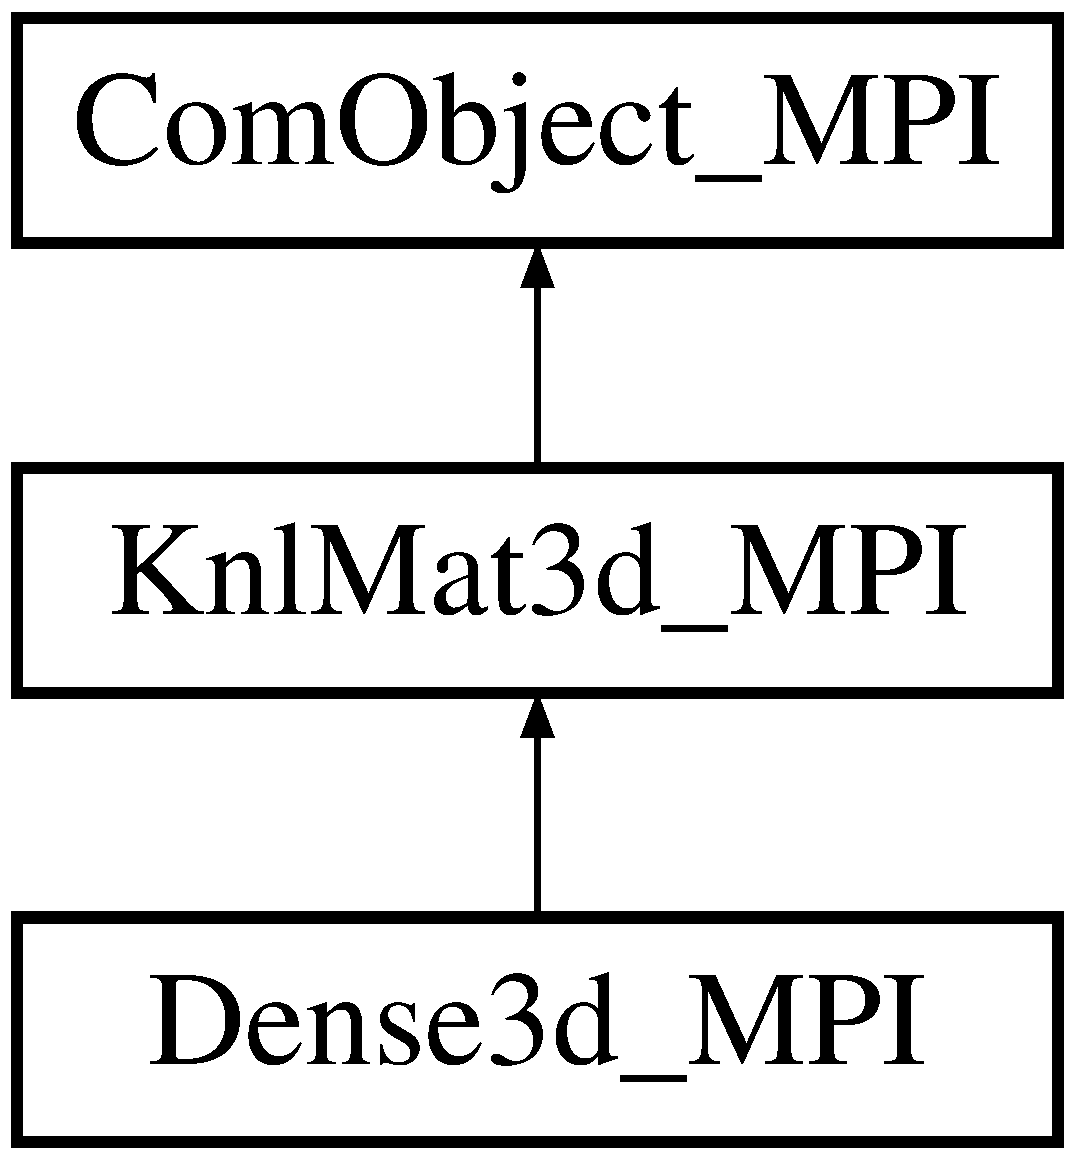
\includegraphics[height=3cm]{classDense3d__MPI}
\end{center}
\end{figure}


\subsection{Detailed Description}
Dense3d\_\-MPI implements setup and evaluate from {\bf Knl\-Mat3d\_\-MPI}{\rm (p.\,\pageref{classKnlMat3d__MPI})} the solver is a \char`\"{}dense\char`\"{} solver - meaning that fmm is not used, and the solution is \char`\"{}exact\char`\"{}. 



Definition at line 32 of file dense3d\_\-mpi.hpp.\subsection*{Public Member Functions}
\begin{CompactItemize}
\item 
{\bf Dense3d\_\-MPI} (const string \&p)
\item 
{\bf $\sim$Dense3d\_\-MPI} ()
\item 
int {\bf setup} ()
\item 
int {\bf evaluate} (Vec srcden, Vec trgval)
\end{CompactItemize}
\subsection*{Protected Attributes}
\begin{CompactItemize}
\item 
Vec {\bf \_\-src\-All\-Pos}
\item 
Vec {\bf \_\-src\-All\-Nor}
\end{CompactItemize}


\subsection{Constructor \& Destructor Documentation}
\index{Dense3d_MPI@{Dense3d\_\-MPI}!Dense3d_MPI@{Dense3d\_\-MPI}}
\index{Dense3d_MPI@{Dense3d\_\-MPI}!Dense3d_MPI@{Dense3d\_\-MPI}}
\subsubsection{\setlength{\rightskip}{0pt plus 5cm}Dense3d\_\-MPI::Dense3d\_\-MPI (const string \& {\em p})}\label{classDense3d__MPI_59f5eb1835ca9679e901a3ed7e570e99_59f5eb1835ca9679e901a3ed7e570e99}


construct Dense3d\_\-MPI using string prefix 

Definition at line 29 of file dense3d\_\-mpi.cpp.

\footnotesize\begin{verbatim}29                                        : 
30   KnlMat3d_MPI(p), _srcAllPos(NULL), _srcAllNor(NULL)
31 {
32 }
\end{verbatim}\normalsize 


\index{Dense3d_MPI@{Dense3d\_\-MPI}!~Dense3d_MPI@{$\sim$Dense3d\_\-MPI}}
\index{~Dense3d_MPI@{$\sim$Dense3d\_\-MPI}!Dense3d_MPI@{Dense3d\_\-MPI}}
\subsubsection{\setlength{\rightskip}{0pt plus 5cm}Dense3d\_\-MPI::$\sim$Dense3d\_\-MPI ()}\label{classDense3d__MPI_465a68462d0c24f1003e280546467196_465a68462d0c24f1003e280546467196}


call $\sim$Knl\-Mat3d\_\-MPI -$>$ $\sim$Com\-Object\_\-MPI.hpp 

Definition at line 34 of file dense3d\_\-mpi.cpp.

References \_\-src\-All\-Pos.

\footnotesize\begin{verbatim}35 {
36   if(_srcAllPos!=NULL) {         VecDestroy(_srcAllPos);  }
37   if(_srcAllNor!=NULL) {         VecDestroy(_srcAllNor);  }
38 }
\end{verbatim}\normalsize 




\subsection{Member Function Documentation}
\index{Dense3d_MPI@{Dense3d\_\-MPI}!evaluate@{evaluate}}
\index{evaluate@{evaluate}!Dense3d_MPI@{Dense3d\_\-MPI}}
\subsubsection{\setlength{\rightskip}{0pt plus 5cm}int Dense3d\_\-MPI::evaluate (Vec {\em srcden}, Vec {\em trgval})\hspace{0.3cm}{\tt  [virtual]}}\label{classDense3d__MPI_b6d6d5d529463497e5bed037a921cfc2_b6d6d5d529463497e5bed037a921cfc2}


Evaluate target values based on source densities and positions using direct evaluation 

Implements {\bf Knl\-Mat3d\_\-MPI} {\rm (p.\,\pageref{classKnlMat3d__MPI_abf7f0a466fbc47db0804a35093c819f_abf7f0a466fbc47db0804a35093c819f})}.

Definition at line 74 of file dense3d\_\-mpi.cpp.

References Knl\-Mat3d\_\-MPI::\_\-knl, \_\-src\-All\-Nor, \_\-src\-All\-Pos, Knl\-Mat3d\_\-MPI::\_\-src\-Nor, Knl\-Mat3d\_\-MPI::\_\-src\-Pos, Knl\-Mat3d\_\-MPI::\_\-trg\-Pos, Kernel3d\_\-MPI::build\-Knl\-Int\-Ctx(), Knl\-Mat3d\_\-MPI::dim(), p\-A, p\-C, Knl\-Mat3d\_\-MPI::proc\-Glb\-Num(), Knl\-Mat3d\_\-MPI::proc\-Lcl\-Num(), Knl\-Mat3d\_\-MPI::src\-DOF(), and Knl\-Mat3d\_\-MPI::trg\-DOF().

\footnotesize\begin{verbatim}75 {
76   //begin
77   // CHECK
78   pA(_srcPos!=NULL && _srcNor!=NULL && _trgPos!=NULL && srcDen!=NULL && trgVal!=NULL);
79   //-----------------------------------
80   int dim  = this->dim();
81   int srcDOF = this->srcDOF();
82   int trgDOF = this->trgDOF();
83   /* Get global number of source positions */
84   int srcGlbNum = procGlbNum(_srcPos);
85   /* Get local number of target positions */
86   int trgLclNum = procLclNum(_trgPos);
87   
88   Vec srcAllPos = _srcAllPos;
89   Vec srcAllNor = _srcAllNor;
90   Vec srcAllDen;
91   /* Create scatter context to scatter source densities to all processors */
92   {
93          VecScatter ctx;
94          pC( VecScatterCreateToAll(srcDen, &ctx, &srcAllDen) );
95          pC( VecScatterBegin(srcDen, srcAllDen, INSERT_VALUES, SCATTER_FORWARD, ctx) );
96          pC( VecScatterEnd(  srcDen, srcAllDen, INSERT_VALUES, SCATTER_FORWARD, ctx) );
97          pC( VecScatterDestroy(ctx) );
98   }
99   
100   Vec trgLclPos = _trgPos;
101   Vec trgLclVal =  trgVal;
102 
103   /* Create matrices for source positions, normals, densities.  See common/nummat.hpp for
104         * more information on matrices */
105   double* srcAllPosArr; pC( VecGetArray(srcAllPos, &srcAllPosArr) );
106   DblNumMat srcAllPosMat(dim, srcGlbNum, false, srcAllPosArr);
107   double* srcAllNorArr; pC( VecGetArray(srcAllNor, &srcAllNorArr) );
108   DblNumMat srcAllNorMat(dim, srcGlbNum, false, srcAllNorArr);
109   double* srcAllDenArr; pC( VecGetArray(srcAllDen, &srcAllDenArr) );
110   DblNumVec srcAllDenVec(srcDOF*srcGlbNum, false, srcAllDenArr);
111 
112   /* Create matrices for target positions and values */
113   double* trgLclPosArr; pC( VecGetArray(trgLclPos, &trgLclPosArr) );
114   DblNumMat trgLclPosMat(dim, trgLclNum, false, trgLclPosArr);
115   double* trgLclValArr; pC( VecGetArray(trgLclVal, &trgLclValArr) );
116   DblNumVec trgLclValVec(trgDOF*trgLclNum, false, trgLclValArr);
117 
118   /* Create an evaluation context and evaluate based on kernel type */
119   DblNumMat inter(trgDOF, srcGlbNum*srcDOF);
120   /* Do multiplication one line of the matrices at a time */
121   for(int i=0; i<trgLclNum; i++) {
122          DblNumMat onePosMat(dim, 1, false, trgLclPosMat.clmdata(i));
123          DblNumVec oneValVec(trgDOF, false, trgLclValVec.data()+trgDOF*i);
124          /* Create kernel multiplier context based on kernel type */
125          pC( _knl.buildKnlIntCtx(srcAllPosMat, srcAllNorMat, onePosMat, inter) );
126          /* Computes 1.0*inter*srcAllDenVec + 0.0*oneValVec = oneValVec */
127          pC( dgemv(1.0, inter, srcAllDenVec, 0.0, oneValVec) );
128   }
129   
130   pC( VecRestoreArray(srcAllPos, &srcAllPosArr) );
131   pC( VecRestoreArray(srcAllNor, &srcAllNorArr) );
132   pC( VecRestoreArray(srcAllDen, &srcAllDenArr) );
133   
134   pC( VecRestoreArray(trgLclPos, &trgLclPosArr) );
135   pC( VecRestoreArray(trgLclVal, &trgLclValArr) );
136   
137   pC( VecDestroy(srcAllDen) );
138   
139   return(0);
140 }
\end{verbatim}\normalsize 


\index{Dense3d_MPI@{Dense3d\_\-MPI}!setup@{setup}}
\index{setup@{setup}!Dense3d_MPI@{Dense3d\_\-MPI}}
\subsubsection{\setlength{\rightskip}{0pt plus 5cm}int Dense3d\_\-MPI::setup ()\hspace{0.3cm}{\tt  [virtual]}}\label{classDense3d__MPI_415266b005d267e801176f27c0434a50_415266b005d267e801176f27c0434a50}


Setup makes sure that all processor have the source positions and noremals scattered to them 

Implements {\bf Knl\-Mat3d\_\-MPI} {\rm (p.\,\pageref{classKnlMat3d__MPI_98f7aa1beebfd344710d076d3d6413a2_98f7aa1beebfd344710d076d3d6413a2})}.

Definition at line 45 of file dense3d\_\-mpi.cpp.

References \_\-\_\-FUNCT\_\-\_\-, \_\-src\-All\-Nor, \_\-src\-All\-Pos, Knl\-Mat3d\_\-MPI::\_\-src\-Nor, Knl\-Mat3d\_\-MPI::\_\-src\-Pos, Knl\-Mat3d\_\-MPI::\_\-trg\-Pos, p\-A, and p\-C.

\footnotesize\begin{verbatim}46 {
47   //begin
48   pA(_srcPos!=NULL && _srcNor!=NULL && _trgPos!=NULL);
49   //--------------------------------------------------------------------------
50   /* Create a Scatter context - copies all source position values to each processor
51         * See http://www-unix.mcs.anl.gov/petsc/petsc-as/snapshots/petsc-current/docs/manualpages/Vec/VecScatterCreateToAll.html */
52   {
53          VecScatter ctx;
54          pC( VecScatterCreateToAll(_srcPos, &ctx, &_srcAllPos) );
55          pC( VecScatterBegin(_srcPos, _srcAllPos, INSERT_VALUES, SCATTER_FORWARD, ctx) );
56          pC( VecScatterEnd(  _srcPos, _srcAllPos, INSERT_VALUES, SCATTER_FORWARD, ctx) );
57          pC( VecScatterDestroy(ctx) );
58   }
59   /* Create a Scatter context - copies all source normal values to each processor */
60   {
61          VecScatter ctx;
62          pC( VecScatterCreateToAll(_srcNor, &ctx, &_srcAllNor) );
63          pC( VecScatterBegin(_srcNor, _srcAllNor, INSERT_VALUES, SCATTER_FORWARD, ctx) );
64          pC( VecScatterEnd(  _srcNor, _srcAllNor, INSERT_VALUES, SCATTER_FORWARD, ctx) );
65          pC( VecScatterDestroy(ctx) );
66   }
67   return(0);
68 }
\end{verbatim}\normalsize 




\subsection{Member Data Documentation}
\index{Dense3d_MPI@{Dense3d\_\-MPI}!_srcAllNor@{\_\-srcAllNor}}
\index{_srcAllNor@{\_\-srcAllNor}!Dense3d_MPI@{Dense3d\_\-MPI}}
\subsubsection{\setlength{\rightskip}{0pt plus 5cm}Vec {\bf Dense3d\_\-MPI::\_\-src\-All\-Nor}\hspace{0.3cm}{\tt  [protected]}}\label{classDense3d__MPI_db2ec95209a80ecf4e75545dbe1bd00d_db2ec95209a80ecf4e75545dbe1bd00d}


all source normals 

Definition at line 39 of file dense3d\_\-mpi.hpp.

Referenced by evaluate(), and setup().\index{Dense3d_MPI@{Dense3d\_\-MPI}!_srcAllPos@{\_\-srcAllPos}}
\index{_srcAllPos@{\_\-srcAllPos}!Dense3d_MPI@{Dense3d\_\-MPI}}
\subsubsection{\setlength{\rightskip}{0pt plus 5cm}Vec {\bf Dense3d\_\-MPI::\_\-src\-All\-Pos}\hspace{0.3cm}{\tt  [protected]}}\label{classDense3d__MPI_864bdce428c7c15d43e08e6733357f13_864bdce428c7c15d43e08e6733357f13}


all source positions 

Definition at line 37 of file dense3d\_\-mpi.hpp.

Referenced by evaluate(), setup(), and $\sim$Dense3d\_\-MPI().

The documentation for this class was generated from the following files:\begin{CompactItemize}
\item 
fmm3d\_\-mpi/{\bf dense3d\_\-mpi.hpp}\item 
fmm3d\_\-mpi/{\bf dense3d\_\-mpi.cpp}\end{CompactItemize}
